% Real-scan example. Top: Liszt, Hungarian Rhapsody No. 2, IMSLP file 300584,
% page 26 (public domain), systems 4 and 5 of the 1050 px model input.
% Bottom: the released constrained-decoding prediction for this page
% (evaluation/predictions/transcoda-constrained.jsonl), converted to Humdrum
% and rendered with Verovio by render_prediction.py, same systems.
% Page OMR-NED 1.28% (evaluation/frozen-public-pages.csv).
\documentclass[border=6pt]{standalone}
% Shared preamble for the README figures. Compile with build.sh.
\usepackage[T1]{fontenc}
\usepackage[sfdefault,scale=0.95,lining]{FiraSans}
\usepackage[scale=0.9]{sourcecodepro}
\usepackage{textcomp}
\usepackage{graphicx}
\usepackage{xcolor}
\usepackage{tikz}
\usepackage{pgfplots}
\pgfplotsset{compat=1.18}
\usetikzlibrary{arrows.meta,positioning,calc,backgrounds,fit,decorations.pathreplacing}
\graphicspath{{assets/}}
\definecolor{ink}{HTML}{1F2328}
\definecolor{muted}{HTML}{59636E}
\definecolor{rule}{HTML}{D1D9E0}
\definecolor{codebg}{HTML}{F6F8FA}
\definecolor{tc}{HTML}{6F42C1}
\definecolor{tclight}{HTML}{C9B6F2}
\definecolor{legato}{HTML}{F0A35E}
\definecolor{smt}{HTML}{9DB4D6}
\color{ink}

\begin{document}
\begin{tikzpicture}[
    lab/.style={font=\small\bfseries, text=muted, anchor=south west, inner sep=0pt},
]
\def\w{17.0cm}
\node[lab] at (0,0.25) {INPUT \textmd{IMSLP scan, public domain}};
\node[anchor=north west, inner sep=0pt] (scan) at (0,0) {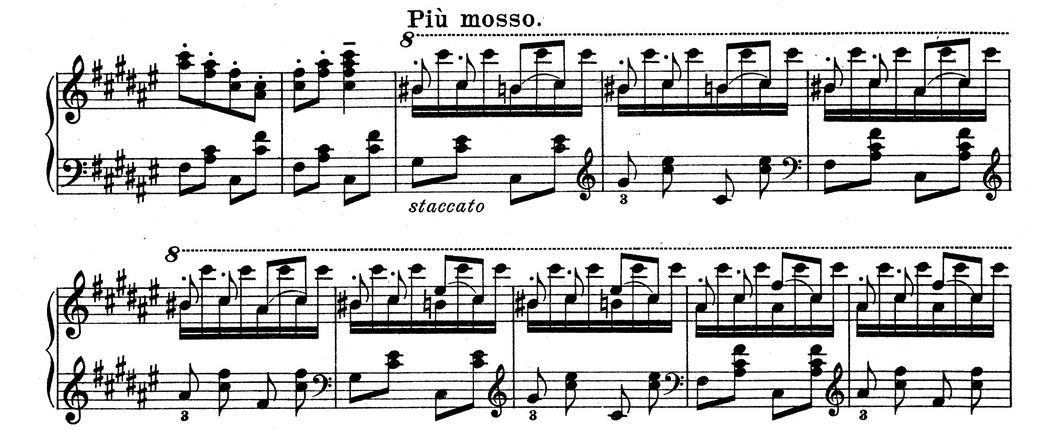
\includegraphics[width=\w]{liszt-p26-systems4-5-scan.png}};
\draw[rule, line width=0.6pt] ($(scan.south west)+(0,-0.3)$) -- ($(scan.south east)+(0,-0.3)$);
\node[lab] (tlab) at ($(scan.south west)+(0,-0.75)$) {OUTPUT \textmd{Transcoda + CD, rendered with Verovio}};
\node[anchor=north west, inner sep=0pt] (out) at ($(tlab.south west)+(0,-0.25)$) {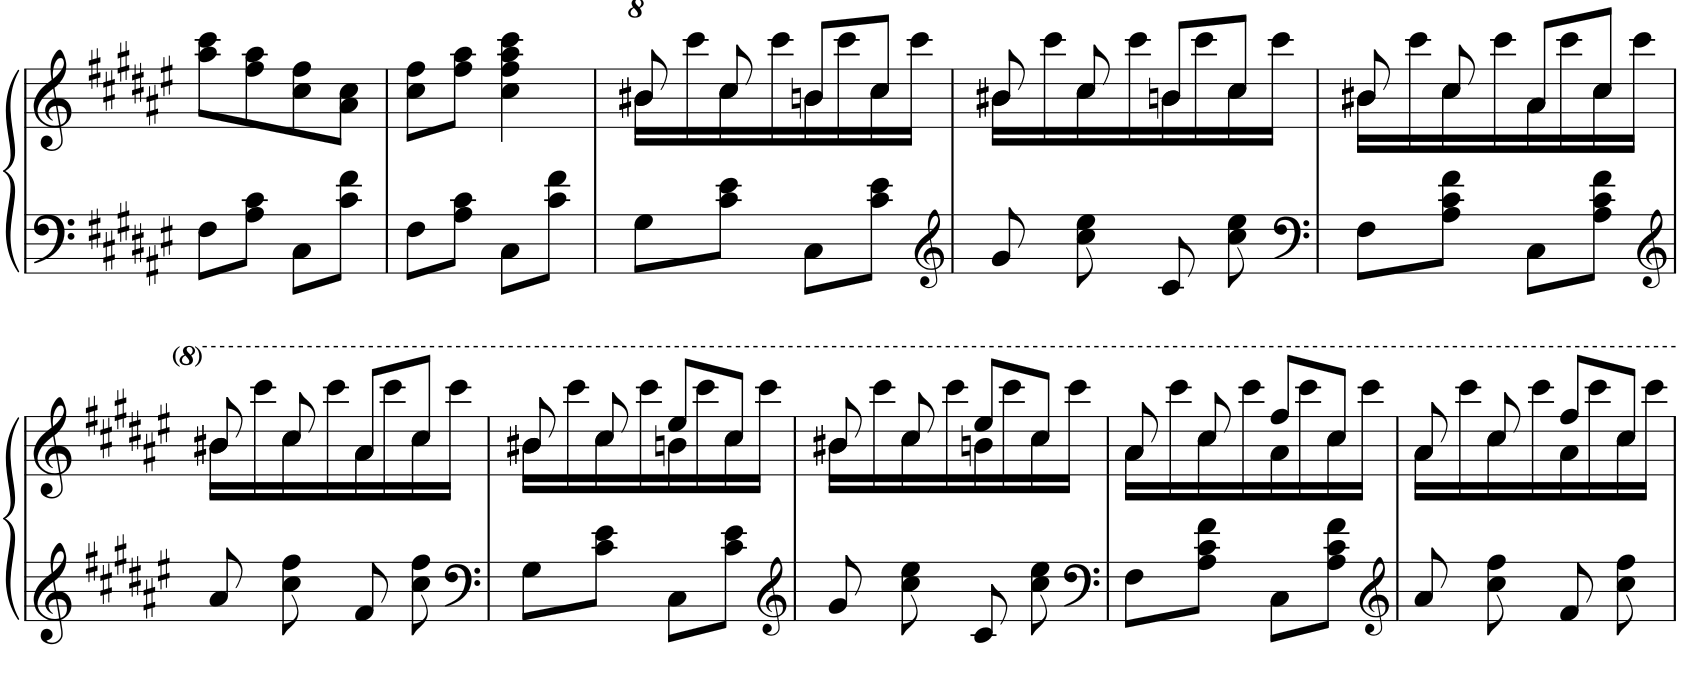
\includegraphics[width=\w]{liszt-p26-systems4-5-transcoda.png}};
\end{tikzpicture}
\end{document}
